\section{Dataset, Applications and Metrics}\label{sects:dataset}
\paragraph{Dataset}
In this section we are going to discuss the dataset and the task that is proposed i.e. Facial Landmark Detection. Our dataset of choice is the 300W dataset \cite{Sagonas13a,Sagonas13b,Sagonas16}. Many other datasets are available, however this one is one of the most popular. 300W comes already split into three parts: Test, Validation and Train each composed of $\sim 600,130,3700$ respectively. Each sample in the dataset is composed of an image and 68 landmark points on the image. The objective is to train a model to match the given points to the image. Fig.~\ref{img:sample} shows two examples.

\paragraph{Applications}
Facial landmark detection can be applied to a variety of important task. For example, \textit{face animation} and \textit{face reenactment} can both exploit the automatic generation of facial landmark. Other important tasks are \textit{driver status tracking} and \textit{emotion classification} and \textit{face recognition} \cite{Khabarlak21}.

\begin{figure}
    \begin{subfigure}{.5\textwidth}
        \centering
        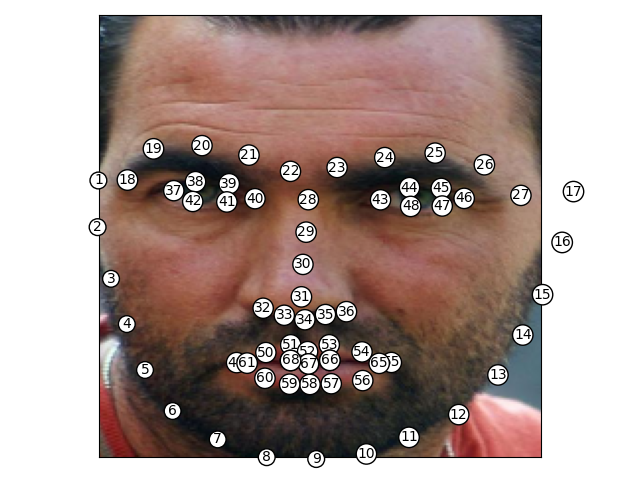
\includegraphics[width=.9\linewidth]{figs/sample1.png}
        \subcaption{Example 1}
    \end{subfigure}
    \begin{subfigure}{.5\textwidth}
        \centering
        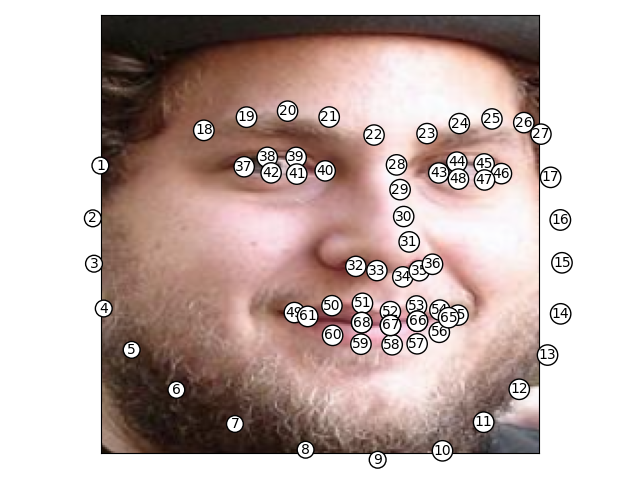
\includegraphics[width=.9\linewidth]{figs/sample2.png}
        \subcaption{Example 2}
    \end{subfigure}
    \caption{Two example with respective annotations from the 300W dataset}
    \label{img:sample}
\end{figure}


\paragraph{Metrics}
The goal of this task is predict accurate landmark on the human face. Therefore, a metric to measure the goodness of a model must take into account this fact. The most popular metric is the \textit{mean error}:
\[ME = \frac{1}{68}\sum_{i=1}^{68}||y_i-\hat{y_i}||\]
Where $y_i \in \mathbb{R}^2$ represent the prediction of i-th landmark and $\hat{y_i} \in \mathbb{R}^2$ represent the true i-th landmark position. Despite seeming perfectly reasonable as metric ME lack an important normalization factor. In fact, An error of $10$ pixel in $4K$ images can be negligeble while the same error on images of size $224\times 224$ can be considered a poor classification. To overcome this issue a normalization factor is introduced $d$. While the importance of $d$ is out of discussion there is not a true consensum among which normalization to adopt. In some cases $d$ is the bounding box dimension, in other cases is the distance between the pupils but, most commonly, it is the distance between the 37-th landmark and 46-th landmark. In this report, we will consider only the latter.
\[NME = \frac{1}{68}\sum_{i=1}^{68}\frac{||y_i-\hat{y_i}||}{d}\]

